%%%%%%%%%%%%%%%%%%%%%PREAMBLE BEGINS%%%%%%%%%%
\documentclass [serif,professionalfont]{beamer}
\usepackage [T1]{fontenc} % Needed for Type1 Concrete
\usepackage {concrete}
% \usepackage{packages}
\usepackage[utf8]{inputenc}
\usepackage{fontawesome,tikz,amsmath,amssymb,graphicx,wrapfig,hyperref,mathtools,multirow,tabularx,mathtools}
\usepackage[normalem]{ulem}%for strikethrough
\usepackage[symbol]{footmisc}%for footnote symbols
\renewcommand{\thefootnote}{\fnsymbol{footnote}}
\usepackage{adjustbox,comment,appendixnumberbeamer}
\usetikzlibrary{petri,automata,positioning,arrows,fit,shapes}
\usetikzlibrary{positioning,shapes.callouts}
\usepackage{rotating}
\usepackage{pdfpages}
\usepackage{algpseudocode}
\usepackage{algorithm}

\useinnertheme{rectangles}%itemized bullets as rectangles
\newcommand{\tup}[1]{\langle#1\rangle}
\newcommand{\TS}{\mathit{TS}}
\newcommand{\fmset}[1]{\{\!\{#1\}\!\}}
\newcommand{\nestTok}{\T}
% \newcommand{\Lstar}{$\mathcal{L}_{UCS}^{1}$}
\newcommand{\LC}{$LTL_{LIA}$}
\newcommand{\Lstar}{$\mathsf{FOTL_1}$}
\newcommand*{\eqdef}{\stackrel{\text{def}}{=}}
\newcommand{\iCar}{\raisebox{-0.9\height}{\faCar}}
%\logo{
\includegraphics[width=1cm]{figures/IITDhL}}
\beamertemplatenavigationsymbolsempty
\setbeamertemplate{footline}[frame number]
\tikzstyle{aldecision} = [diamond, draw, fill=blue!20,
text width=4.5em, text badly centered, node distance=2.5cm, inner sep=0pt]
\tikzstyle{alblock} = [rectangle, draw, fill=blue!20,
text width=5em, text centered, rounded corners, minimum height=4em]
\tikzstyle{line} = [draw, very thick, color=black!50, -latex']
\tikzstyle{allibrary} = [draw, ellipse,fill=red!20, node distance=2.5cm,
minimum height=2em]
%for live windows
\usepackage{pgfgantt}
\definecolor{foobarblue}{RGB}{0,153,255}
\newganttchartelement{foobar}{
foobar/.style={
shape=rectangle,
inner sep=0pt,
draw=foobarblue!50!black,
very thick,
fill=white
}
}
\newcommand\textganttbar[4]{%
    \ganttfoobar{#1}{#3}{#4}
    \ganttfoobar[inline,bar label font=\footnotesize]
    {#2}{#3}{#4}
}
%\setbeamertemplate{blocks}[rounded][shadow=true]
%\setbeamercolor{block body}{bg=cyan!10}
\newcommand{\hlfancy}[2]{\sethlcolor{#1}\hl{#2}}

\usepackage{smartdiagram}
\usesmartdiagramlibrary{additions}
\smartdiagramset{module minimum width=3cm,text width=3cm}
%%%%%%%%%%%%%%%%%%%%%%%%%%%%%%%%%%%%%%%%%%%%%%%%%%%%%%%%%%%%%%%%


\title{Formal verification of infinite state systems with \textcolor{purple}{unbounded} agents}


\author[ Tephilla Prince]{Tephilla Prince \\Indian Institute of Technology Dharwad \\\vspace{3em} Supervisors:\\Prof. Ramchandra Phawade\\Prof. S. Sheerazuddin}


\date{\tiny{05/03/2026}}
\usepackage[style=authortitle,backend=bibtex]{biblatex}
\bibliography{mybibliography.bib}
\renewbibmacro*{cite:title}{%
  \printtext[bibhyperref]{%
    \printfield[citetitle]{labeltitle}%
    \setunit{\space}%
    \printtext[parens]{\printdate}%
  }%
}
%%%%%%%%%%%%%%%%%%%%%PREAMBLE ENDS%%%%%%%%%%%%


\begin{document}
% \input{macros}
\begin{frame}
    \titlepage
\end{frame}

\begin{frame}
    \begin{figure}
        \centering
        \smartdiagramset{module minimum width=2.5cm,text width=2cm}
        \smartdiagramadd[circular diagram]{
            Gather Requirements,Design,Code,Testing,Maintenance
        }{}
        \caption{Traditional Software Development Life Cycle}
        \label{fig:sdlc}
    \end{figure}
\end{frame}

\begin{frame}{Error Costs}
    \centering
    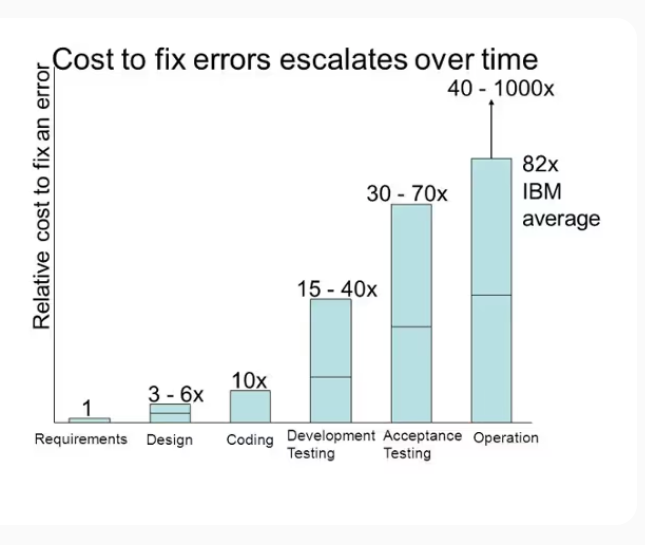
\includegraphics[width=0.6\textwidth]{figures/errorcost}

    \tiny{J. Stecklein, “Error cost escalation through the project life cycle, 2010}
\end{frame}

\begin{frame}{What is model checking?}
    \begin{center}


        Does  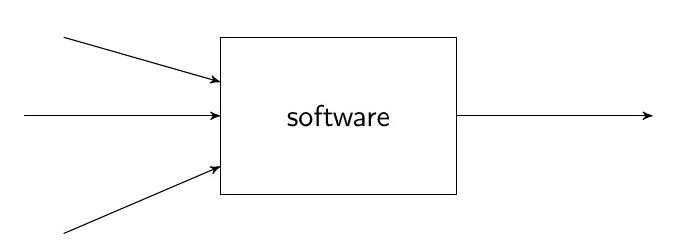
\includegraphics[width=10em]{figures/softwareio} satisfy 
\includegraphics[width=2em]{figures/requirements} ?

        
\includegraphics[width=2em]{figures/updownarrow}

        Does  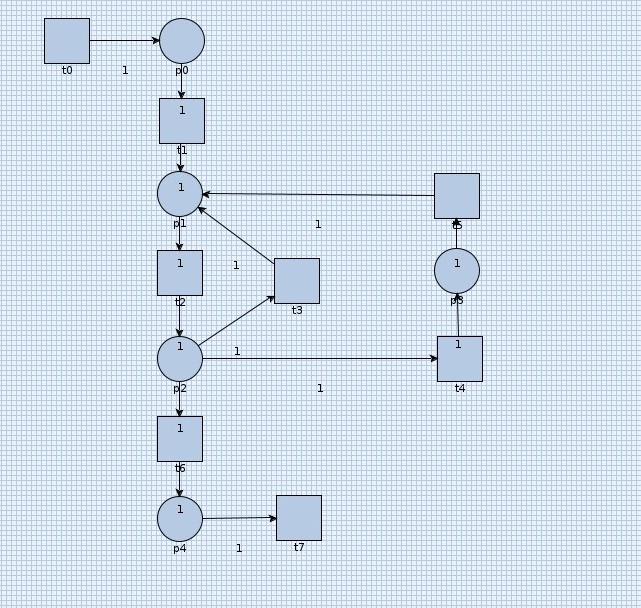
\includegraphics[width=5em]{figures/SchedulerPN} satisfy 
\includegraphics[width=5em]{figures/spec1} ?
    \end{center}
\end{frame}

\begin{frame}
    \frametitle{\small{Running example: Unbounded Client-Server System (UCS)}}

    \begin{tikzpicture}[scale=0.45, note/.style={rectangle callout, fill=####1}]
        \visible<1>{

            \node[draw,text width=5cm, draw=green!15, fill=green!15] at (13,12) {An empty Parking Lot waits for vehicles};
        }

        \node   at  (1,1)   [rectangle, thick, draw=yellow!20, fill=black!30,inner sep=0pt,minimum height=4cm, minimum width=5.5cm] (bga){};
        %Row0
        \node   at  (5,3.5)     [rectangle, thick, draw=yellow!90, fill=black!5,inner sep=0pt,minimum height=1cm, minimum width=0.8cm] (s1){};

        \node   at  (2.5,3.5)   [rectangle, thick, draw=yellow!90, fill=black!5,inner sep=0pt,minimum height=1cm, minimum width=0.8cm] (s2){};

        \node   at  (0,3.5)     [rectangle, thick, draw=yellow!90, fill=black!5,inner sep=0pt,minimum height=1cm, minimum width=0.8cm] (s3){};

        \node   at  (-2.5,3.5)  [rectangle, thick, draw=yellow!90, fill=black!5,inner sep=0pt,minimum height=1cm, minimum width=0.8cm] (s4){};

        %closed gate
        \node   at  (6.6,1.8)   [rectangle, thick, draw=green!90, fill=black!60,inner sep=0pt,minimum height=1cm, minimum width=0.2cm] (gate){};

        %Row1
        \node   at  (5,-0.5)    [rectangle, thick, draw=yellow!90, fill=black!5,inner sep=0pt,minimum height=1cm, minimum width=0.8cm] (s5){};

        \node   at  (2.5,-0.5)  [rectangle, thick, draw=yellow!90, fill=black!5,inner sep=0pt,minimum height=1cm, minimum width=0.8cm] (s6){};

        \node   at  (0,-0.5)    [rectangle, thick, draw=yellow!90, fill=black!5,inner sep=0pt,minimum height=1cm, minimum width=0.8cm] (s7){};

        \node   at  (-2.5,-0.5)     [rectangle, thick, draw=yellow!90, fill=black!5,inner sep=0pt,minimum height=1cm, minimum width=0.8cm] (s8){};

        \node   at  (6,7.5)     [circle, thick, draw=red!50,inner sep=0pt,minimum height=1cm, minimum width=1cm] (parking){\large P};

        \node   at  (6,5.5)     [rectangle, thick, draw=red!50,inner sep=0pt,minimum height=-.2cm, minimum width=0.2cm] (hidden){};

        \draw (parking) -- (hidden);

        %car outside gate       
        \visible<2,3>{
            \node   at  (8,1.8)     [rectangle, thick,inner sep=0pt,minimum height=1cm, minimum width=0.2cm] (car){{\iCar}};
        }

        %Park Request
        \visible<2>{
            \node [note=yellow!50, callout absolute pointer={(8,2)}] at (12,4) {Can I park here?};
        }

        %Accept request      
        \visible<3>{
            \node [note=blue!20, callout absolute pointer={(6,6)}] at (12,4){Yeah, come in!};
            \node  at  (6.6,1.8)   [rectangle, thick, draw=green!30, fill=green!30,inner sep=0pt,minimum height=1cm, minimum width=0.2cm] (gate){};}

        %Allocated Parking Lot       
        \visible<4>{
            \node     at  (5,3.5)     [rectangle, thick, draw=yellow!90, fill=black!5,inner sep=0pt,minimum height=1cm, minimum width=0.8cm] (s1){\iCar };
            \node [note=blue!20, callout absolute pointer={(6,6)}] at (12,4){Parking Lot allocated};
        }

        %Multiple Requests waiting
        \visible<5>{
            %car outside gate

            \node[draw,text width=4cm, draw=green!15, fill=green!15] at (13,12) {Unbounded number of parking requests};

            \node  at  (5,3.5)     [rectangle, thick, draw=yellow!90, fill=black!5,inner sep=0pt,minimum height=1cm, minimum width=0.8cm] (s1){\iCar };
            \node   at  (8,1.8)     [rectangle, thick,inner sep=0pt,minimum height=1cm, minimum width=0.2cm] (car1){\iCar };
            \node   at  (10,1.8)    [rectangle, thick,inner sep=0pt,minimum height=1cm, minimum width=0.2cm] (car2){\iCar };
            \node   at  (12,1.8)    [rectangle, thick,inner sep=0pt,minimum height=1cm, minimum width=0.2cm] (car3){\iCar };
            \node   at  (14,1.8)    [rectangle, thick,inner sep=0pt,minimum height=1cm, minimum width=0.2cm] (car4){\iCar };
            \node   at  (16,1.8)    [rectangle, thick,inner sep=0pt,minimum height=1cm, minimum width=0.2cm] (car1){$\ldots$};
            \node [note=yellow!50, callout absolute pointer={(8,2)}] at (12,4) {Can I park here?};
        }

        \visible<6>{

            \node[draw,text width=3cm, draw=green!15, fill=green!15] at (13,12) {No parking space};

        }

        %Parking lot full
        \visible<6,7,8,9>{
            %Row0
            \node   at  (5,3.5)     [rectangle, thick, draw=yellow!90, fill=black!5,inner sep=0pt,minimum height=1cm, minimum width=0.8cm] (s1){\iCar };

            \node   at  (2.5,3.5)   [rectangle, thick, draw=yellow!90, fill=black!5,inner sep=0pt,minimum height=1cm, minimum width=0.8cm] (s2){\iCar };

            \node   at  (0,3.5)     [rectangle, thick, draw=yellow!90, fill=black!5,inner sep=0pt,minimum height=1cm, minimum width=0.8cm] (s3){\iCar };

            \node   at  (-2.5,3.5)  [rectangle, thick, draw=yellow!90, fill=black!5,inner sep=0pt,minimum height=1cm, minimum width=0.8cm] (s4){\iCar };


            %Row1
            \node   at  (5,-0.5)    [rectangle, thick, draw=yellow!90, fill=black!5,inner sep=0pt,minimum height=1cm, minimum width=0.8cm] (s5){\iCar };

            \node   at  (2.5,-0.5)  [rectangle, thick, draw=yellow!90, fill=black!5,inner sep=0pt,minimum height=1cm, minimum width=0.8cm] (s6){\iCar };

            \node   at  (0,-0.5)    [rectangle, thick, draw=yellow!90, fill=black!5,inner sep=0pt,minimum height=1cm, minimum width=0.8cm] (s7){\iCar };

            \node   at  (-2.5,-0.5)     [rectangle, thick, draw=yellow!90, fill=black!5,inner sep=0pt,minimum height=1cm, minimum width=0.8cm] (s8){\iCar };

        }

        %Request when Full
        \visible<7>{

            \node   at  (8,1.8)     [rectangle, thick,inner sep=0pt,minimum height=1cm, minimum width=0.2cm] (car){\iCar };
            \node [note=yellow!50, callout absolute pointer={(8,2.5)}] at (12,4) {Can I park here?};

        }

        %Reject request when full
        \visible<8>{
            \node [note=blue!20, callout absolute pointer={(6,6)}] at (12,4){No};
            \node   at  (6.6,1.8)   [rectangle, thick, draw=red!30, fill=red!30,inner sep=0pt,minimum height=1cm, minimum width=0.2cm] (gate){};
            \node   at  (8,1.8)     [rectangle, thick,inner sep=0pt,minimum height=1cm, minimum width=0.2cm] (car){\iCar };
        }

        %Vehicle Exit Request
        \visible<9>{
            %        \node  at  (5,3.5)     [rectangle, thick, draw=yellow!90, fill=black!5,inner sep=0pt,minimum height=1cm, minimum width=0.5cm] (s1){\iCar };
            \node [note=yellow!50, callout absolute pointer={(5,3.5)}] at (12,4) {I'm exiting};

        }
        %Deallocate Parking lot 
        \visible<10>{
            \node [note=blue!20, callout absolute pointer={(6,6)}] at (12,4){Parking Lot Deallocated};
            \node   at  (5,3.5)     [rectangle, thick, draw=yellow!90, fill=black!5,inner sep=0pt,minimum height=1cm, minimum width=0.8cm] (s1){};

            \node   at  (2.5,3.5)   [rectangle, thick, draw=yellow!90, fill=black!5,inner sep=0pt,minimum height=1cm, minimum width=0.8cm] (s2){\iCar };

            \node   at  (0,3.5)     [rectangle, thick, draw=yellow!90, fill=black!5,inner sep=0pt,minimum height=1cm, minimum width=0.8cm] (s3){\iCar };

            \node   at  (-2.5,3.5)  [rectangle, thick, draw=yellow!90, fill=black!5,inner sep=0pt,minimum height=1cm, minimum width=0.8cm] (s4){\iCar };


            %Row1
            \node   at  (5,-0.5)    [rectangle, thick, draw=yellow!90, fill=black!5,inner sep=0pt,minimum height=1cm, minimum width=0.8cm] (s5){\iCar };

            \node   at  (2.5,-0.5)  [rectangle, thick, draw=yellow!90, fill=black!5,inner sep=0pt,minimum height=1cm, minimum width=0.8cm] (s6){\iCar };

            \node   at  (0,-0.5)    [rectangle, thick, draw=yellow!90, fill=black!5,inner sep=0pt,minimum height=1cm, minimum width=0.8cm] (s7){\iCar };

            \node   at  (-2.5,-0.5)     [rectangle, thick, draw=yellow!90, fill=black!5,inner sep=0pt,minimum height=1cm, minimum width=0.8cm] (s8){\iCar };
        }

        %Vehicle Request to exit and incoming parking request.
        \visible<11>{

            \node[draw,text width=10cm, draw=green!15] at (5,12) {- single server-multiple client system\\- \colorbox{green!30}{unbounded} clients of the same type};
            \node [note=yellow!50, callout absolute pointer={(5,-0.5)}] at (12,0) {I'm exiting};
            \node   at  (8,1.8)     [rectangle, thick,inner sep=0pt,minimum height=1cm, minimum width=0.2cm] (car){\iCar };
            \node   at  (10,1.8)    [rectangle, thick,inner sep=0pt,minimum height=1cm, minimum width=0.2cm] (car2){\iCar };
            \node [note=yellow!50, callout absolute pointer={(8,2.5)}] at (12,4) {Can I park here?};


            \node   at  (5,3.5)     [rectangle, thick, draw=yellow!90, fill=black!5,inner sep=0pt,minimum height=1cm, minimum width=0.8cm] (s1){};

            \node   at  (2.5,3.5)   [rectangle, thick, draw=yellow!90, fill=black!5,inner sep=0pt,minimum height=1cm, minimum width=0.8cm] (s2){\iCar };

            \node   at  (0,3.5)     [rectangle, thick, draw=yellow!90, fill=black!5,inner sep=0pt,minimum height=1cm, minimum width=0.8cm] (s3){\iCar };

            \node   at  (-2.5,3.5)  [rectangle, thick, draw=yellow!90, fill=black!5,inner sep=0pt,minimum height=1cm, minimum width=0.8cm] (s4){\iCar };


            %Row1
            \node   at  (5,-0.5)    [rectangle, thick, draw=yellow!90, fill=black!5,inner sep=0pt,minimum height=1cm, minimum width=0.8cm] (s5){\iCar };

            \node   at  (2.5,-0.5)  [rectangle, thick, draw=yellow!90, fill=black!5,inner sep=0pt,minimum height=1cm, minimum width=0.8cm] (s6){\iCar };

            \node   at  (0,-0.5)    [rectangle, thick, draw=yellow!90, fill=black!5,inner sep=0pt,minimum height=1cm, minimum width=0.8cm] (s7){\iCar };

            \node   at  (-2.5,-0.5)     [rectangle, thick, draw=yellow!90, fill=black!5,inner sep=0pt,minimum height=1cm, minimum width=0.8cm] (s8){\iCar };
        }

    \end{tikzpicture}
\end{frame}



\begin{frame}{Case Study Parking System: Server behaviour}
    \begin{figure}[!ht]
        \centering
        \scalebox{0.7}{\input{figures/state_diag_aps}}
    \end{figure}
\end{frame}

\begin{frame}{Case Study Parking System: Client behaviour}
    \begin{figure}[!ht]
        \centering
        \scalebox{0.7}{\input{figures/state_diag_vehicle}}
    \end{figure}
\end{frame}


\begin{frame}\frametitle{Research Questions}
    \begin{enumerate}
        \item How do we formally verify UCS?

        \item How do we formally model UCS?


        \item How do we express properties of client-server systems naturally?
              \begin{enumerate}
                  \item Do existing logics suffice?
                  \item What additional properties are interesting in the context of unbounded client-server systems?
              \end{enumerate}\pause

        \item Are there formal verification tools for UCS? Can we add to the repertoire?
              \begin{enumerate}
                  \item How are existing tools different, unique? Is another tool necessary?
              \end{enumerate}
    \end{enumerate}
\end{frame}


\begin{frame}
    \frametitle{\small{Challenge 1: Modelling UCS \colorbox{green!30}{using Petri Nets}}}
    \begin{figure}[!ht]
        \begin{center}
            \input{figures/fig_aps_names}
        \end{center}
    \end{figure}
\end{frame}


\begin{frame}\frametitle{Challenge 1: Modelling UCS \colorbox{green!30}{using Petri Nets}}

    \begin{columns}[T] % align columns
        \begin{column}{.5\textwidth}
            \begin{figure}
                \begin{center}
                    \scalebox{0.8}{\input{figures/fig_aps_pn}}
                \end{center}
            \end{figure}
        \end{column}
        \hfill
        \begin{column}{.5\textwidth}
            Finite sets of atomic client propositions $P_c$ and server propositions $P_s$:
            \small{
                \begin{align*}
                    P_c
                     & =\{parking\_requested (PR),            \\
                     & \qquad~occupy\_parking\_lot (OP),      \\
                     & \qquad~parking\_unavailable (PU),      \\
                     & \qquad~exit\_successfully (ES),        \\
                     & \qquad~exited\_unsuccessfully (EU)\}   \\
                    P_s
                     & =\{server\_ready (SR),                 \\
                     & \qquad~server\_busy(SB),               \\
                     & \qquad~request\_granted (RG),          \\
                     & \qquad~request\_rejected(RR),          \\
                     & \qquad~deallocate\_parking\_lot (DP)\}
                \end{align*}
            }
        \end{column}%
    \end{columns}
\end{frame}


\begin{frame}{}
    \centering
    \huge{Question: What properties of the system are we interested in?}
\end{frame}



\begin{frame}{Properties }
    \begin{enumerate}

        \item \textcolor{blue}{Is the number of clients occupying parking lots = number of requests granted always?}
        \item[] $ G (\#p_{OP}= \#p_{RG})$
            % \item[] There is no counterexample for this property for upto bound $50$
            \pause

        \item \textcolor{blue}{Consider the property, $p_{PR}+p_{OP}+p_{ES} = 1$, which is an invariant.}

        \item[] $G(\#p_{PR} + \#p_{OP} + \#p_{ES} =1)$.
            \pause
        \item \textcolor{blue}{Is the number of rejected requests greater than the number of accepted requests at some point?}


        \item[]
            $F(\#p_{EU} > \#p_{ES})$.
    \end{enumerate}
\end{frame}

\begin{frame}{Linear Temporal Logic with Integer Arithmetic {\LC}}

    In {\LC},there are two types of atomic formulas:
    \begin{enumerate}
        \item $P_s$ - describing basic server properties, which are propositional constants and can be used to describe the transitions of the net
        \item $\beta \in \Delta$, the set of client formulas
    \end{enumerate}
    \begin{equation}
        \begin{split}
            \alpha , \hat{\alpha}&::= \#p \mid \mathfrak{c} \mid (\mathfrak{c} \ast \#p ) \mid  (\#p \ast \mathfrak{c}) \mid (\alpha + \hat{\alpha} ) \mid (\alpha - \hat{\alpha})\\ \nonumber
            \beta &::=  (\alpha < \hat{\alpha}) \mid (\alpha > \hat{\alpha}) \mid (\alpha \le \hat{\alpha}) \mid  (\alpha \ge \hat{\alpha}) \mid (\alpha=\hat{\alpha})
        \end{split}
    \end{equation}


    \noindent where $p \in P_c$, the set of client propositions and $\mathfrak{c} \in \mathbb{Z}^+$.% is a non-negative integer, as noted above. %While $\Delta$ does not contain an explicit $=$ operator, it is natural to express equality of $p(x)$ and $q(x)$ as follows: 

    %$ ((\#x) p(x) <= q(x) \land \neg ((\#x) q(x) > p(x)))$.

    \noindent The set of server formulas $\Psi$ are defined as follows:

    \[\psi::= q \in P_s \mid \beta \in \Delta
        \mid \lnot \psi  \mid \psi\lor\psi^{\prime}   \mid \psi\land\psi^{\prime}  \mid  X \psi  \mid F \psi\mid G \psi \mid \psi U  \psi^{\prime}\]
    where $\psi, \psi^{\prime} \in \Psi$.
    Modalities X, F, G and $U$ are the usual modal operators: Next, Eventually, Globally and Until, respectively.

    % In $\mathcal{L}_{C}$,
    % there are two types of atomic formulas:
    % \begin{enumerate}
    %     \item  $P_s$ - describing basic server properties, which are propositional constants
    %     \item $\beta \in \Delta$, the set of client formulas, which is formally given by:
    % \end{enumerate}

    % \begin{equation}
    %     \begin{split}
    %         \alpha , \hat{\alpha}&::= \#p \mid \mathfrak{c} \mid (\mathfrak{c} \#p ) \mid  (\#p \mathfrak{c}) \mid (\alpha + \hat{\alpha} ) \mid (\alpha - \hat{\alpha})\\ \nonumber
    %         \beta &::=  (\alpha \le \hat{\alpha}) \mid (\alpha > \hat{\alpha}) \mid (\alpha=\hat{\alpha})
    %     \end{split}
    % \end{equation}
    % where $p \in P_c$, the set of client propositions and $\mathfrak{c} \in \mathbb{Z}^+$

    % The set of server formulas $\psi \in \Psi$ are defined as follows:

    % \[\psi::= q \mid \beta \mid \lnot \psi  \mid \psi\lor\psi^{\prime}   \mid \psi\land\psi^{\prime}  \mid  X \psi  \mid F \psi\mid G \psi \mid \psi U  \psi^{\prime}\]
    % where $q \in P_s$, $\beta \in \Delta$.

\end{frame}



\begin{frame}
    \frametitle{BMC vs $2D$-BMC}

    \begin{columns}[T] % align columns
        \begin{column}{.4\textwidth}
            %\color{red}\rule{\linewidth}{4pt}
            %Left Part
            \begin{figure}
                \begin{center}
                    \scalebox{0.5}{\input{figures/formula_unfold_grid_fig5}}
                    %\caption{$\lambda + \kappa = k, k \geq 0$, $\lambda$ : time instance, $\kappa$: no. of tokens}
                \end{center}
            \end{figure}
        \end{column}%
        \hfill%
        \begin{column}{.6\textwidth}
            \begin{itemize}
                \item In BMC, ``We ask whether the system $M$ has any counterexample of length $k$ to (property) $\psi$. This bounded problem is encoded into SAT.'' - A.Biere\footnote{Linear Encodings of Bounded LTL Model Checking, Biere et al, LMCS, 2006}
                \item In $2D$-BMC, we ask whether the system $M$ has any counterexample to $\psi$, of length $\lambda$ and number of tokens $\kappa$  and encode this bounded problem into SMT.
            \end{itemize}
        \end{column}%	
    \end{columns}
\end{frame}



%2DBMC workflow and unfolding
\begin{frame}
    \frametitle{The $2D$-BMC strategy}
    \resizebox{0.9\textwidth}{0.9\textheight}{
        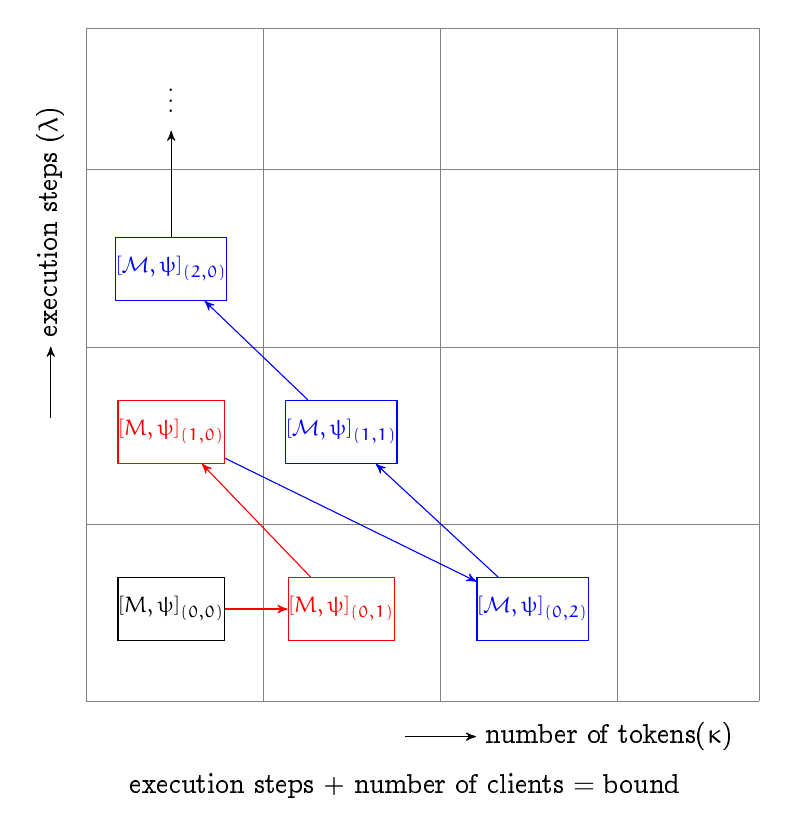
\begin{tikzpicture}[>=stealth,scale=0.9]
            \tikzset{
                %Define standard arrow tip
                >=stealth',
                %Define style for boxes
                punkt/.style={
                        rectangle,
                        rounded corners,
                        draw=black, very thick,
                        text width=8.5em,
                        minimum height=2em,
                        text centered},
                % Define arrow style
                pil/.style={
                        ->,
                        thick,
                        shorten <=2pt,
                        shorten >=2pt,}
            }
            \tikzstyle{aldecision} = [diamond, draw, fill=blue!20, text width=4.5em, text badly centered, node distance=2.5cm, inner sep=0pt]
            \tikzstyle{alblock} = [rectangle, draw, fill=blue!20, text width=5em, text centered, rounded corners, minimum height=4em]
            \tikzstyle{line} = [draw, very thick, color=black!50, -latex']
            \tikzstyle{allibrary} = [draw, ellipse,fill=red!20, node distance=2.5cm, minimum height=2em]


            \foreach \i in {0,2.5,5,7.5,9.5} {
                    \draw[gray,very thin] (0,\i) -- (9.5,\i);
                    \draw[gray,very thin] (\i,0) -- (\i,9.5);
                }
            \draw[->] (-.5,4) -- (-.5,5) node[above] {\begin{turn}{90} execution steps ($\lambda$)\end{turn}};
            \draw[->] (4.5,-0.5) -- (5.5,-0.5) node[right] {number of tokens($\kappa$)};
            \visible<1->{		\node[draw=none] at (4.5,-1.2) (key) {execution steps + number of clients $=$ bound};
            }

            \begin{scope}[every node/.style={
                            circle,draw,
                            minimum size=.8cm,
                            align=center,
                            font=\footnotesize,
                            inner sep=0pt
                        }]

                %column lambda=0
                \visible<1->{		\node[rectangle] at (1.2,1.3) (00) {$[M,\psi]_{(0,0)}$};
                }
                %k=1 lambda=0 kappa=1 
                \visible<2->{		\node[rectangle,red] at (3.6,1.3) (01) {$[M,\psi]_{(0,1)}$};
                    \draw[red,->] (00) -- (01);
                }
                %k=1 lambda=1 kappa=0 
                \visible<3->{		\node[rectangle,red] at (1.2,3.8) (10) {$[M,\psi]_{(1,0)}$};
                    %	\draw[red,->] (00) -- (10);

                    \draw[red,->] (01) -- (10);
                }

                \visible<4->{
                    \node[rectangle,blue] at (1.2,6.1) (20) {$[\mathcal{M},\psi]_{(2,0)}$};
                    \node[rectangle,draw=none,rotate=90] at (1.2,8.5) (30) {$\cdots$};
                    \node[rectangle,blue] at (3.6,3.8) (11) {$[\mathcal{M},\psi]_{(1,1)}$};
                    %\node[rectangle,draw=none,rotate=90] at (3.6,6.1) (21) {$\cdots$};
                    %column lambda=2 
                    \node[rectangle,blue] at (6.3,1.3) (02) {$[\mathcal{M},\psi]_{(0,2)}$};
                    %\node[rectangle,draw=none] at (6.3,3.8) (12) {$\cdots$};
                    %column lambda=3
                    %\node[rectangle,draw=none] at (8.5,1.3) (03) {$\cdots$}; 
                    %\draw[blue,->] (10) -- (20);
                    %\draw[blue,->] (01) -- (11);	
                    %\draw[blue,->] (01) -- (02);

                    \draw[blue,->] (10) -- (02);
                    \draw[blue,->] (02) -- (11);
                    \draw[blue,->] (11) -- (20);

                    \draw[->] (20) -- (30);

                    %\draw[->] (20) -- (30); 
                    %\draw[->] (11) -- (21); 
                    %\draw[->] (11) -- (12);
                    %\draw[->] (02) -- (03);



                }

            \end{scope}
        \end{tikzpicture}
    }
\end{frame}





% \begin{frame}{$2$D-BMC Algorithm}
%     \begin{figure}[!ht]
%         \centering
%         \scalebox{0.7}{\input{figures/formula_unfold_grid_fig5}}
%         \caption{Unfolding of the encoded formula  $[\mathcal{M},\psi]_{(\lambda,\kappa)}$ with respect to $\lambda$ (execution steps) and $\kappa$ (number of tokens)}

%         \label{2dbmcunfolding}
%     \end{figure}
% \end{frame}



\begin{frame}{Tool Architecture}
    \begin{figure}[!ht]
        \centering
        \scalebox{0.5}{\input{figures/fig_arch}}
        \caption{DCModelChecker  architecture}

    \end{figure}
\end{frame}

\begin{frame}{Experimental Results}
    \begin{figure}[ht]
        \centering
        \scalebox{0.4}{
\includegraphics{figures/FCPlots/Angiogenesis-PT-01_FCPlot.eps}}
        \caption{Verification of FireabilityCardinality Properties with bound 5 and 10}
        \label{FCAngioPlot}


    \end{figure}

    \tiny{Verified against 16 Benchmarks from Model Checking Contest 2025}
\end{frame}



\begin{frame}{Experimental Results}
    \begin{table}[ht]
        \centering
        \resizebox{0.7\columnwidth}{!}{

            \begin{tabular}{|c|c|c|c|c|}
                \hline
                \multirow{2}{*}{Model} & \multicolumn{4}{c|}{Execution Times(ms)}                                                   \\
                \cline{2-5}
                                       & DCModelChecker 1.0                       & DCModelChecker 2.0 & ITS-Tools & Tapaal         \\
                \hline
                Parity                 & \textbf{0.010}                           & 0.40               & 0.933     & 0.02           \\
                \hline
                PGCD                   & \textbf{0.019}                           & 0.98               & 1.487     & 0.07           \\
                \hline
                Process                & 0.033                                    & 0.85               & 1.201     & \textbf{1e-05} \\
                \hline
                CryptoMiner            & 0.036                                    & 0.64               & 0.957     & \textbf{7e-06} \\
                \hline
                Murphy                 & 0.031                                    & 0.83               & 1.161     & \textbf{8e-06} \\
                \hline
            \end{tabular}
        }
        \caption{Results of Comparative Experiments on Unbounded PNs}
        \label{table:unboundedpn}

    \end{table}

\end{frame}




\begin{frame}
    \frametitle{Contributions}
    \begin{itemize}
        \item Part 1: Verification of Unbounded Client-Server (UCS) using Petri Nets and Linear Temporal Logic with integer arithmetic using $2$D-BMC

    \end{itemize}

\end{frame}
\begin{frame}\frametitle{Challenge 2: Modelling an UCS with \colorbox{green!30}{distinguishable clients}}
    \huge{What if clients needed to be distinguished?}
\end{frame}

\begin{frame}
    \frametitle{Running example}

    \begin{tikzpicture}[scale=0.45, note/.style={rectangle callout, fill=####1}]
        \visible<1>{

            \node[draw,text width=5cm, draw=green!15, fill=green!15] at (13,12) {An empty Parking Lot waits for vehicles};
        }

        \node   at  (1,1)   [rectangle, thick, draw=yellow!20, fill=black!30,inner sep=0pt,minimum height=4cm, minimum width=5.5cm] (bga){};
        %Row0
        \node   at  (5,3.5)     [rectangle, thick, draw=yellow!90, fill=black!5,inner sep=0pt,minimum height=1cm, minimum width=0.8cm] (s1){};

        \node   at  (2.5,3.5)   [rectangle, thick, draw=yellow!90, fill=black!5,inner sep=0pt,minimum height=1cm, minimum width=0.8cm] (s2){};

        \node   at  (0,3.5)     [rectangle, thick, draw=yellow!90, fill=black!5,inner sep=0pt,minimum height=1cm, minimum width=0.8cm] (s3){};

        \node   at  (-2.5,3.5)  [rectangle, thick, draw=yellow!90, fill=black!5,inner sep=0pt,minimum height=1cm, minimum width=0.8cm] (s4){};

        %closed gate
        \node   at  (6.6,1.8)   [rectangle, thick, draw=green!90, fill=black!60,inner sep=0pt,minimum height=1cm, minimum width=0.2cm] (gate){};

        %Row1
        \node   at  (5,-0.5)    [rectangle, thick, draw=yellow!90, fill=black!5,inner sep=0pt,minimum height=1cm, minimum width=0.8cm] (s5){};

        \node   at  (2.5,-0.5)  [rectangle, thick, draw=yellow!90, fill=black!5,inner sep=0pt,minimum height=1cm, minimum width=0.8cm] (s6){};

        \node   at  (0,-0.5)    [rectangle, thick, draw=yellow!90, fill=black!5,inner sep=0pt,minimum height=1cm, minimum width=0.8cm] (s7){};

        \node   at  (-2.5,-0.5)     [rectangle, thick, draw=yellow!90, fill=black!5,inner sep=0pt,minimum height=1cm, minimum width=0.8cm] (s8){};

        \node   at  (6,7.5)     [circle, thick, draw=red!50,inner sep=0pt,minimum height=1cm, minimum width=1cm] (parking){\large P};

        \node   at  (6,5.5)     [rectangle, thick, draw=red!50,inner sep=0pt,minimum height=-.2cm, minimum width=0.2cm] (hidden){};

        \draw (parking) -- (hidden);

        %car outside gate       
        \visible<2,3>{
            \node   at  (8,1.8)     [rectangle, thick,inner sep=0pt,minimum height=1cm, minimum width=0.2cm] (car){{\iCar}1};
        }

        %Park Request
        \visible<2>{
            \node [note=yellow!50, callout absolute pointer={(8,2)}] at (12,4) {Can I park here?};
        }

        %Accept request      
        \visible<3>{
            \node [note=blue!20, callout absolute pointer={(6,6)}] at (12,4){Yeah, come in!};
            \node  at  (6.6,1.8)   [rectangle, thick, draw=green!30, fill=green!30,inner sep=0pt,minimum height=1cm, minimum width=0.2cm] (gate){};}

        %Allocated Parking Lot       
        \visible<4>{
            \node     at  (5,3.5)     [rectangle, thick, draw=yellow!90, fill=black!5,inner sep=0pt,minimum height=1cm, minimum width=0.8cm] (s1){\iCar 1};
            \node [note=blue!20, callout absolute pointer={(6,6)}] at (12,4){Parking Lot allocated};
        }

        %Multiple Requests waiting
        \visible<5>{
            %car outside gate

            \node[draw,text width=4cm, draw=green!15, fill=green!15] at (13,12) {Unbounded number of parking requests};

            \node  at  (5,3.5)     [rectangle, thick, draw=yellow!90, fill=black!5,inner sep=0pt,minimum height=1cm, minimum width=0.8cm] (s1){\iCar 1};
            \node   at  (8,1.8)     [rectangle, thick,inner sep=0pt,minimum height=1cm, minimum width=0.2cm] (car1){\iCar 2};
            \node   at  (10,1.8)    [rectangle, thick,inner sep=0pt,minimum height=1cm, minimum width=0.2cm] (car2){\iCar 3};
            \node   at  (12,1.8)    [rectangle, thick,inner sep=0pt,minimum height=1cm, minimum width=0.2cm] (car3){\iCar 4};
            \node   at  (14,1.8)    [rectangle, thick,inner sep=0pt,minimum height=1cm, minimum width=0.2cm] (car4){\iCar 5};
            \node   at  (16,1.8)    [rectangle, thick,inner sep=0pt,minimum height=1cm, minimum width=0.2cm] (car1){$\ldots$};
            \node [note=yellow!50, callout absolute pointer={(8,2)}] at (12,4) {Can I park here?};
        }

        \visible<6>{

            \node[draw,text width=3cm, draw=green!15, fill=green!15] at (13,12) {No parking space};

        }

        %Parking lot full
        \visible<6,7,8,9>{
            %Row0
            \node   at  (5,3.5)     [rectangle, thick, draw=yellow!90, fill=black!5,inner sep=0pt,minimum height=1cm, minimum width=0.8cm] (s1){\iCar 1};

            \node   at  (2.5,3.5)   [rectangle, thick, draw=yellow!90, fill=black!5,inner sep=0pt,minimum height=1cm, minimum width=0.8cm] (s2){\iCar 3};

            \node   at  (0,3.5)     [rectangle, thick, draw=yellow!90, fill=black!5,inner sep=0pt,minimum height=1cm, minimum width=0.8cm] (s3){\iCar 98};

            \node   at  (-2.5,3.5)  [rectangle, thick, draw=yellow!90, fill=black!5,inner sep=0pt,minimum height=1cm, minimum width=0.8cm] (s4){\iCar 2};


            %Row1
            \node   at  (5,-0.5)    [rectangle, thick, draw=yellow!90, fill=black!5,inner sep=0pt,minimum height=1cm, minimum width=0.8cm] (s5){\iCar 10};

            \node   at  (2.5,-0.5)  [rectangle, thick, draw=yellow!90, fill=black!5,inner sep=0pt,minimum height=1cm, minimum width=0.8cm] (s6){\iCar 23};

            \node   at  (0,-0.5)    [rectangle, thick, draw=yellow!90, fill=black!5,inner sep=0pt,minimum height=1cm, minimum width=0.8cm] (s7){\iCar 11};

            \node   at  (-2.5,-0.5)     [rectangle, thick, draw=yellow!90, fill=black!5,inner sep=0pt,minimum height=1cm, minimum width=0.8cm] (s8){\iCar 94};

        }

        %Request when Full
        \visible<7>{

            \node   at  (8,1.8)     [rectangle, thick,inner sep=0pt,minimum height=1cm, minimum width=0.2cm] (car){\iCar 99};
            \node [note=yellow!50, callout absolute pointer={(8,2.5)}] at (12,4) {Can I park here?};

        }

        %Reject request when full
        \visible<8>{
            \node [note=blue!20, callout absolute pointer={(6,6)}] at (12,4){No};
            \node   at  (6.6,1.8)   [rectangle, thick, draw=red!30, fill=red!30,inner sep=0pt,minimum height=1cm, minimum width=0.2cm] (gate){};
            \node   at  (8,1.8)     [rectangle, thick,inner sep=0pt,minimum height=1cm, minimum width=0.2cm] (car){\iCar 99};
        }

        %Vehicle Exit Request
        \visible<9>{
            %        \node  at  (5,3.5)     [rectangle, thick, draw=yellow!90, fill=black!5,inner sep=0pt,minimum height=1cm, minimum width=0.5cm] (s1){\iCar 1};
            \node [note=yellow!50, callout absolute pointer={(5,3.5)}] at (12,4) {I'm exiting};

        }
        %Deallocate Parking lot 
        \visible<10>{
            \node [note=blue!20, callout absolute pointer={(6,6)}] at (12,4){Parking Lot Deallocated};
            \node   at  (5,3.5)     [rectangle, thick, draw=yellow!90, fill=black!5,inner sep=0pt,minimum height=1cm, minimum width=0.8cm] (s1){};

            \node   at  (2.5,3.5)   [rectangle, thick, draw=yellow!90, fill=black!5,inner sep=0pt,minimum height=1cm, minimum width=0.8cm] (s2){\iCar 3};

            \node   at  (0,3.5)     [rectangle, thick, draw=yellow!90, fill=black!5,inner sep=0pt,minimum height=1cm, minimum width=0.8cm] (s3){\iCar 98};

            \node   at  (-2.5,3.5)  [rectangle, thick, draw=yellow!90, fill=black!5,inner sep=0pt,minimum height=1cm, minimum width=0.8cm] (s4){\iCar 2};


            %Row1
            \node   at  (5,-0.5)    [rectangle, thick, draw=yellow!90, fill=black!5,inner sep=0pt,minimum height=1cm, minimum width=0.8cm] (s5){\iCar 10};

            \node   at  (2.5,-0.5)  [rectangle, thick, draw=yellow!90, fill=black!5,inner sep=0pt,minimum height=1cm, minimum width=0.8cm] (s6){\iCar 23};

            \node   at  (0,-0.5)    [rectangle, thick, draw=yellow!90, fill=black!5,inner sep=0pt,minimum height=1cm, minimum width=0.8cm] (s7){\iCar 11};

            \node   at  (-2.5,-0.5)     [rectangle, thick, draw=yellow!90, fill=black!5,inner sep=0pt,minimum height=1cm, minimum width=0.8cm] (s8){\iCar 94};
        }

        %Vehicle Request to exit and incoming parking request.
        \visible<11>{
            %\frametitle{A motivating example: single server-multiple client system (clients of the same type)}
            \node[draw,text width=10cm, draw=green!15] at (5,12) {- single server-multiple client system\\- \colorbox{green!30}{unbounded distinguishable} clients of the same type};
            %\frametitle{Parking System handles one request at a time}
            \node [note=yellow!50, callout absolute pointer={(5,-0.5)}] at (12,0) {I'm exiting};
            \node   at  (8,1.8)     [rectangle, thick,inner sep=0pt,minimum height=1cm, minimum width=0.2cm] (car){\iCar 99};
            \node   at  (10,1.8)    [rectangle, thick,inner sep=0pt,minimum height=1cm, minimum width=0.2cm] (car2){\iCar 100};
            \node [note=yellow!50, callout absolute pointer={(8,2.5)}] at (12,4) {Can I park here?};


            \node   at  (5,3.5)     [rectangle, thick, draw=yellow!90, fill=black!5,inner sep=0pt,minimum height=1cm, minimum width=0.8cm] (s1){};

            \node   at  (2.5,3.5)   [rectangle, thick, draw=yellow!90, fill=black!5,inner sep=0pt,minimum height=1cm, minimum width=0.8cm] (s2){\iCar 3};

            \node   at  (0,3.5)     [rectangle, thick, draw=yellow!90, fill=black!5,inner sep=0pt,minimum height=1cm, minimum width=0.8cm] (s3){\iCar 98};

            \node   at  (-2.5,3.5)  [rectangle, thick, draw=yellow!90, fill=black!5,inner sep=0pt,minimum height=1cm, minimum width=0.8cm] (s4){\iCar 2};


            %Row1
            \node   at  (5,-0.5)    [rectangle, thick, draw=yellow!90, fill=black!5,inner sep=0pt,minimum height=1cm, minimum width=0.8cm] (s5){\iCar 10};

            \node   at  (2.5,-0.5)  [rectangle, thick, draw=yellow!90, fill=black!5,inner sep=0pt,minimum height=1cm, minimum width=0.8cm] (s6){\iCar 23};

            \node   at  (0,-0.5)    [rectangle, thick, draw=yellow!90, fill=black!5,inner sep=0pt,minimum height=1cm, minimum width=0.8cm] (s7){\iCar 11};

            \node   at  (-2.5,-0.5)     [rectangle, thick, draw=yellow!90, fill=black!5,inner sep=0pt,minimum height=1cm, minimum width=0.8cm] (s8){\iCar 94};
        }

    \end{tikzpicture}
\end{frame}


\begin{frame}\frametitle{Modelling an Unbounded Client-Server (UCS)}
    \begin{columns}[T] % align columns
        \begin{column}{.5\textwidth}
            \begin{figure}
                \begin{center}
                    \scalebox{0.8}{\input{figures/fig_aps}}
                \end{center}
            \end{figure}
        \end{column}
        \hfill
        \begin{column}{.5\textwidth}
            Finite sets of atomic client propositions $P_c$ and server propositions $P_s$:
            \small{
                \begin{align*}
                    P_c
                     & =\{parking\_requested (PR),            \\
                     & \qquad~occupy\_parking\_lot (OP),      \\
                     & \qquad~parking\_unavailable (PU),      \\
                     & \qquad~exit\_successfully (ES),        \\
                     & \qquad~exited\_unsuccessfully (EU)\}   \\
                    P_s
                     & =\{server\_ready (SR),                 \\
                     & \qquad~server\_busy(SB),               \\
                     & \qquad~request\_granted (RG),          \\
                     & \qquad~request\_rejected(RR),          \\
                     & \qquad~deallocate\_parking\_lot (DP)\}
                \end{align*}
            }
        \end{column}%
    \end{columns}
\end{frame}



\begin{frame}{}
    \centering
    \huge{Question: What properties of the system are we interested in?}
\end{frame}



\begin{frame}{Properties}
    \begin{enumerate}

        \item When a vehicle requests a parking space, it is always the case that for every vehicle, it eventually exits the system, either successfully after being granted a parking space, or unsuccessfully, when its request is denied.
              \pause
              \begin{align*}
                   & \mathbf{G}_s(\forall x) \Big( parking\_requested(x) \Rightarrow                \\
                   & \qquad\mathbf{F}_c~ (exit\_successfully(x)~\lor~exit\_unsuccessfully(x)) \Big)
              \end{align*}
              \pause
        \item It is always the case that if the client occupies a parking lot, it will eventually exit the parking lot. \pause
              \begin{align*}
                   & \mathbf{G}_s(\forall x) \Big(occupy\_parking\_lot(x)\Rightarrow \mathbf{F}_c(exit\_successfully(x))\Big)
              \end{align*}
              %We expect that this property will hold true. 
    \end{enumerate}
\end{frame}


\begin{frame}{Properties}
    \begin{enumerate}
        \setcounter{enumi}{2}
        \item There may be clients whose requests are rejected.\pause
              \begin{align*}
                   & \mathbf{G}_s(\exists x) \big(parking\_requested(x) \land \mathbf{F}_c (exit\_unsuccessfully(x))\big)
              \end{align*}
              \pause
        \item There may be clients who have requested for parking and who wait in the parking unavailable state until they are able to exit the system.\pause
              \begin{align*}
                   & \mathbf{G}_s(\exists x) \bigg( parking\_requested(x)~\land                                 \\
                   & \mathbf{F}_c \big( parking\_unavailable(x)~\mathbf{U}_c~exit\_unsuccessfully(x)\big)\bigg)
              \end{align*}
    \end{enumerate}
\end{frame}


\begin{frame}
    \frametitle{The proposed logic: The Monodic\footnote{Decidable fragment of first-order temporal logics. Hodkinson et al. '00} Logic {\Lstar}}

    \subsection{Syntax}
    \visible<1->{
        The set of \colorbox{green!30}{client formulae} $\Delta$:
        \[\Delta ::= p(x)\mid \lnot\alpha \mid \alpha\lor\beta \mid  \alpha \land \beta \mid \mathbf{X}_c \alpha\mid \mathbf{F}_c\alpha \mid \mathbf{G}_c \alpha \mid \alpha ~\mathbf{U}_c~ \beta\]

        where $\alpha,\beta \in \Delta$ and $p\in P_c$, the set of atomic client propositions.
    }

    %\visible<2->{Let $\Phi=\{(\exists x)\alpha,(\forall x)\alpha \mid \alpha \in \Delta\}$.}

    \visible<2->{
        The set of  \colorbox{green!30}{server formulae} $\Psi$:
        \begin{equation}
            \begin{split}
                \Psi ::= & q \mid \lnot \psi \mid (\exists x)\alpha \mid (\forall x)\alpha \mid\psi_1 \lor \psi_2 \mid \psi_1\land \psi_2 \mid\\ \nonumber
                & \mathbf{X_s} \psi \mid \mathbf{F_s} \psi \mid \mathbf{G_s}\psi \mid \psi_1 ~\mathbf{U_s}~\psi_2
            \end{split}
        \end{equation}
        where $\psi, \psi_1, \psi_2 \in \Psi$ and $q \in P_s$, the set of atomic server propositions, $\alpha \in \Delta$.
    }

\end{frame}




\begin{frame}
    \frametitle{The Monodic Logic {\Lstar} (contd)}

    \[\psi = (\exists x)(\exists y) \bigg(\big(PR(x) \land PR(y)\big)\land \mathbf{F_c}\big(ES(x) \land ES(y)\big)\bigg)\]
    \begin{itemize}[<+->]
        \item Is $\psi\in$ {\Lstar}?
        \item \textcolor{purple}{Answer: No. \textbf{not a well formed formula} in {\Lstar}}% $\psi$ is a non-monodic formula which is \textbf{not a well formed formula} in {\Lstar}.}
              %\end{itemize}
              %\begin{itemize}    
              %\item[] Note: 
              %\item[-]  In server formula $\Psi$ every variable is bounded.

              %\item[-] In {\Lstar}, the quantifier depth is atmost one. 
              %\item[-] Quantifier alternation is not allowed.
    \end{itemize}
\end{frame}



\begin{frame}\frametitle{Recall: our model}
    \begin{columns}[T] % align columns
        \begin{column}{.5\textwidth}
            \begin{figure}
                \begin{center}
                    \scalebox{0.8}{\input{figures/fig_aps}}
                \end{center}
            \end{figure}
        \end{column}
        \hfill
        \begin{column}{.5\textwidth}
            Atomic client propositions $P_c$ and server propositions $P_s$:
            \small{
                \begin{align*}
                    P_c
                     & =\{parking\_requested (PR),            \\
                     & \qquad~occupy\_parking\_lot (OP),      \\
                     & \qquad~parking\_unavailable (PU),      \\
                     & \qquad~exit\_successfully (ES),        \\
                     & \qquad~exited\_unsuccessfully (EU)\}   \\
                    P_s
                     & =\{server\_ready (SR),                 \\
                     & \qquad~server\_busy(SB),               \\
                     & \qquad~request\_granted (RG),          \\
                     & \qquad~request\_rejected(RR),          \\
                     & \qquad~deallocate\_parking\_lot (DP)\}
                \end{align*}
            }
        \end{column}
    \end{columns}
\end{frame}


\begin{frame}{Snapshots of the system + live windows}


    \begin{ganttchart}[
            vgrid,hgrid,
            progress label text=\relax,
            x unit=10mm,
            title height=1,
            foobar top shift=.15,
            foobar height=.70
        ]{0}{2}
        \visible<1>{\textganttbar{Client 1}{$p_{PR}$}{0}{0} }
        \visible<2>{\textganttbar{Client 1}{$p_{PR}$}{0}{0}  \textganttbar{}{$p_{OP}$}{1}{1}}
        \visible<3>{
            \textganttbar{Client 1}{$p_{PR}$}{0}{0}  \textganttbar{}{$p_{OP}$}{1}{1} \textganttbar{}{$p_{OP}$}{2}{2}\\
            \textganttbar{Client 2}{$p_{PR}$}{2}{2}
        }



        \begin{scope}[yshift=0.33cm]
            \draw[->] (0,0) -- (3.7,0);
            \draw ([yshift=-3pt]0,0) -- ++([yshift=6pt]0,0) node[xshift=45pt, yshift=15pt, above] {time instance $\rightarrow$};
            \draw ([yshift=-3pt]1,0) -- ++([yshift=6pt]0,0) node[xshift=-10pt, above] {$0$};
            \visible<2->{
                \draw ([yshift=-3pt]2,0) -- ++([yshift=6pt]0,0) node[xshift=-10pt, above] {$1$};}
            \visible<3->{\draw ([yshift=-3pt]3,0) -- ++([yshift=6pt]0,0) node[xshift=-10pt, above] {$2$};}
        \end{scope}
    \end{ganttchart}
\end{frame}




\begin{frame}{Snapshots of the system + live windows (contd)}
    \begin{columns}[T] % align columns
        \begin{column}{.5\textwidth}
            \begin{figure}
                \begin{center}
                    \scalebox{0.8}{\input{figures/live_windows_overlap}}
                \end{center}
            \end{figure}
        \end{column}%
        \hfill%
        \begin{column}{.5\textwidth}
            \begin{itemize}
                \item $4$ distinguishable clients, with overlapping \emph{live windows}, with the bound $5$.
                \item client $1$ is at $p_{PR}$ at instance $0$. i.e, $PR(x)$ is satisfied in client $1$ at instance $0$.
                \item For client $1$, the \emph{left boundary} is at instance $0$ and its \emph{right boundary} is at instance $2$.
            \end{itemize}
        \end{column}
    \end{columns}
\end{frame}




\begin{frame}{Formally speaking...}
    \begin{itemize}
        \item Let $CN$ be a \colorbox{green!30}{countable set of client names}. \pause
        \item Let $CS = (Q,\Sigma,\delta,I,F)$ be a \colorbox{green!30}{finite state machine describing the client behaviour}. \pause
        \item Let $L:Q \to 2^{P_c}$ be the labelling function of each client state  $q \in Q$ in terms of a \colorbox{green!30}{subset of propositions $P_c$ true in that state}. \pause

        \item Let $\mathfrak{Z}:CN \times \mathbb{N}_0 \to Q$ be a partial mapping describing the local state of each client $a \in CN$ at an instance $i \in \mathbb{N}_0$. \pause
              \item[-]For instance, $\mathfrak{Z}(a,i)\in q$, means that the \colorbox{green!30}{local state of each client $a$ at instance $i$ is state $q$}, where $q \in Q$.
    \end{itemize}
\end{frame}


\begin{frame}{Formally speaking...}
    A model is a triple $M=(\nu,V,\xi)$ where
    \begin{itemize}
        \item $\nu$ gives the \colorbox{green!30}{local behaviour of the server} as follows:

              $\nu=\nu_0\nu_1\nu_2\ldots$, where for all $0 \le i$, $\nu_i \subseteq P_s$ \pause

        \item $V$ gives the \colorbox{green!30}{set of live agents (clients) at each instance}.

              $V=V_0V_1V_2\ldots$, where for all $0 \le i$, $V_i$ is a finite subset of $CN$, gives the set of live agents at the $i$th instance.

              For every $0\le i$, $V_i$ and $V_{i+1}$ satisfy  the following properties:
              \begin{enumerate}
                  \item if $V_i \subseteq V_{i+1}$ then for every $a \in V_{i+1}-V_i$ such that $\mathfrak{Z}(a,i+1)\in I$.
                  \item if $V_{i+1}\subseteq V_i$ then for every $a \in V_i-V_{i+1}$ such that $\mathfrak{Z}(a,i)\in F$.
              \end{enumerate} \pause

        \item $\xi=\xi_0\xi_1\xi_2\cdots$, where for all $0 \le i$, $\xi_i:V_i\to 2^{P_c}$ gives \colorbox{green!30}{the properties satisfied by each live agent at $i$th instance.}
              \item[]Also, $L(\mathfrak{Z}(a,i))=\xi_i(a)$. %Alternatively, $\xi_i$ can be given as $\xi_i:V_i\times P_c \to\{\top,\bot\}$. %, an equivalent form.
    \end{itemize}
\end{frame}




\begin{frame}{Semantics}
    \visible<1->{
        $M,i \models (\exists x)\alpha$ iff $\exists a\in CN$, $a \in V_i$ and $M,[x\mapsto a],i\models_x \alpha$.
    }

    \visible<2->{

        $M,i \models^{k} (\exists x)\alpha$ iff $\exists a\in CN$, $a \in V_i$ and $M,[x\mapsto a],i\models^{k}_x \alpha$.
    }

    \begin{columns}[T] % align columns
        \begin{column}{.4\textwidth}
            \visible<3->{
                \begin{figure}
                    \begin{center}
                        \scalebox{0.8}{\input{figures/live_windows_overlap_line}}
                    \end{center}
                \end{figure}
            }
        \end{column}%
        \hfill%
        \begin{column}{.6\textwidth}
            \visible<4->{
                \begin{itemize}
                    \item[]
                        Given $\alpha=OP(x) \lor PR(x)$ and  $CN=\{1,2\}$.
                \end{itemize}
            }
            \visible<5->{
                \begin{itemize}
                    \item $M,0 \models^{k} (\exists x)(OP(x) \lor PR(x))$.
                    \item $M,1 \models^{k} (\exists x)(OP(x) \lor PR(x))$.
                    \item $M,2 \models^{k} (\exists x)(OP(x) \lor PR(x))$.
                \end{itemize}
            }
        \end{column}%
    \end{columns}
\end{frame}



\begin{frame}{Bounded Semantics}
    $M,i \models^{k} (\forall x)\alpha$ iff $\forall a\in CN$, if $a \in V_i$ then $M,[x\mapsto a],i\models^{k}_x \alpha$
    \begin{columns}[T]
        \begin{column}{.4\textwidth}
            \begin{figure}
                \begin{center}
                    \scalebox{0.8}{\input{figures/live_windows_overlap_line}}
                \end{center}
            \end{figure}
        \end{column}
        \hfill
        \begin{column}{.6\textwidth}
            \begin{itemize}
                \item[]
                    Given $\alpha=ES(x)$ and  $CN=\{1,2\}$.
                \item $M,0 \not\models^{k} (\exists x)(ES(x))$.
                \item $M,1 \not\models^{k} (\exists x)(ES(x))$.
                \item $M,2 \not\models^{k} (\exists x)(ES(x))$.
            \end{itemize}
        \end{column}
    \end{columns}
\end{frame}



\begin{frame}{Bounded Semantics}
    $M,i\models^{k} \mathbf{F_s}\psi$ iff $\exists j: i \le j \le k$ , $M,j\models^{k} \psi$.

    Given $\psi= (\exists x)ES(x)$.
    \begin{columns}[T]
        \begin{column}{.5\textwidth}
            \begin{figure}
                \begin{center}
                    \scalebox{0.8}{\input{figures/live_windows_overlap_line_3}}
                \end{center}
                \caption{Snapshot with 4 clients}
                \label{fig:4clientssnp}
            \end{figure}
        \end{column}
        \hfill
        \begin{column}{.5\textwidth}
            \begin{figure}
                \begin{center}
                    \scalebox{0.8}{\input{figures/live_windows_overlap_line}}
                \end{center}
                \caption{Snapshot with 2 clients}
                \label{fig:2clientssnap}
            \end{figure}
        \end{column}
    \end{columns} \pause
    As shown above $M,5\models^{k} \mathbf{F_s}(\exists x)ES(x)$.
\end{frame}



\begin{frame}
    \frametitle{Implementation}

    Verifying $G_s \exists x (F_c(p_0(x)))$


    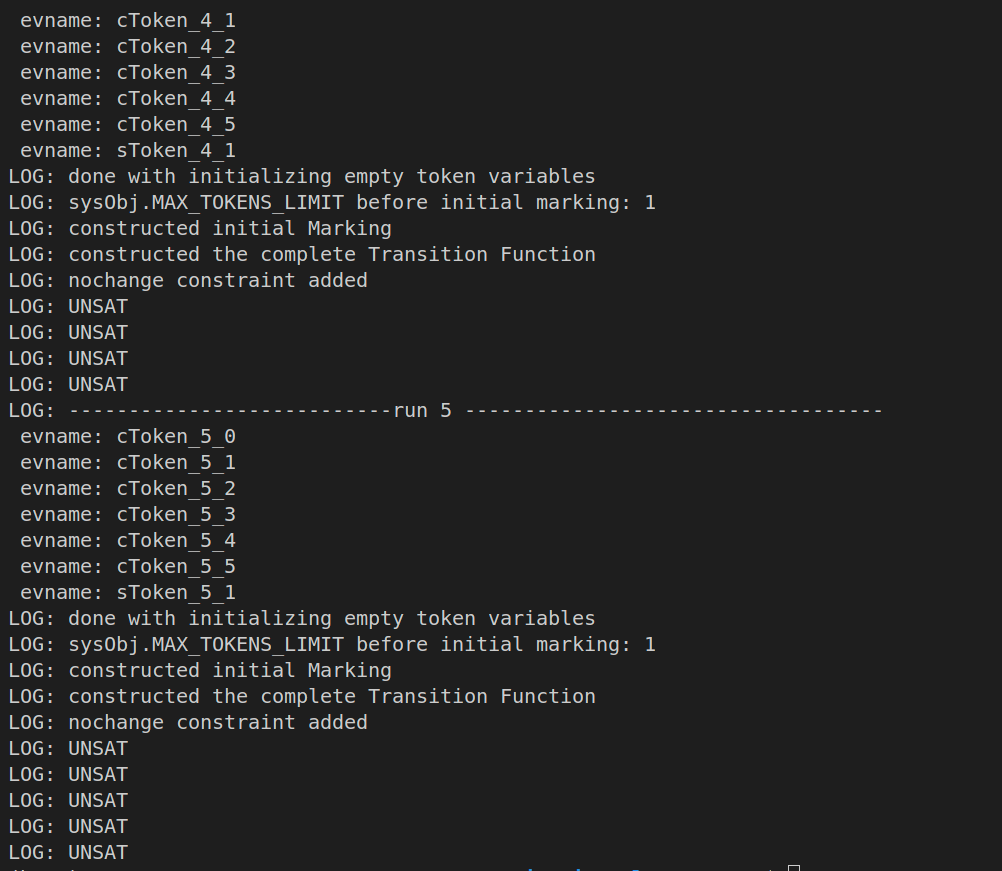
\includegraphics[width=9cm]{figures/result.png}


\end{frame}


\begin{frame}
    \frametitle{Contributions}
    \begin{itemize}
        \item Part 1: Verification of UCS using Petri Nets and {\LC}
        \item Part 2: Verification of UCS with distinguishable clients using $\nu$-nets and properties specified in {\Lstar}
    \end{itemize}

\end{frame}



\begin{frame}\frametitle{Challenge 3: Modelling an UCS with \colorbox{green!30}{internal structure}}
    \huge{What if clients had an internal structure?}
\end{frame}


\begin{frame}
    \input{figures/2_cpn}%client Petri net
\end{frame}
\begin{frame}
    \input{figures/2_spn}%server Petri net
\end{frame}


\begin{frame}{Modelling UCS via Elementary Object Systems}
    \input{figures/2_ucseos}%EOS for UCS 
\end{frame}



\begin{frame}
    \begin{block}{Question: What properties of the system are we interested in?}
        \begin{itemize}
            \item \textbf{Reachability:} Is $\mu_1={\tup{\mathtt{SR},\fmset{\mathtt{client1CR},\mathtt{client2CR}}}}$ a reachable marking?
            \item \textbf{Coverability:} Given $\mu_1={\tup{\mathtt{SR},\fmset{\mathtt{client1CR},\mathtt{client2OP}}}}$ and $\mu_2={\tup{\mathtt{SR },\fmset{\mathtt{client1OP},\mathtt{client2CR},\mathtt{client3OP}}}}$.
            \item[] Then, is $\mu_1 \preceq \mu_2$?
        \end{itemize}
    \end{block}

\end{frame}




\includepdf[pages={8-33}]{eosslides.pdf}


\begin{frame}
    \frametitle{Contributions}
    \begin{itemize}
        \item Part 1: Verification of Unbounded Client-Server (UCS) using Petri Nets and Linear Temporal Logic with integer arithmetic
        \item Part 2: Verification of UCS with distinguishable clients using $\nu$-nets and properties specified in monodic First Order Logic
        \item Part 3: Verification of UCS where the clients have internal structure using Elementary Object Systems and properties specified in Linear Temporal Logic
    \end{itemize}

\end{frame}

\begin{frame}{List of publications:}
    \begin{enumerate}
        \item Ramchandra Phawade, Tephilla Prince, S. Sheerazuddin:
              Bounded Model Checking for Unbounded Client Server Systems. Arxiv (2026),  submitted to TopNOC
        \item Ramchandra Phawade, Tephilla Prince, S. Sheerazuddin: Verification of Unbounded Client-Server Systems with Distinguishable Clients Arxiv (2026), submitted to TopNOC
        \item   Tephilla Prince:
              On Verifying Unbounded Client-Server Systems. Springer EUMAS 2023: 465-471
        \item   Francesco Di Cosmo, Tephilla Prince:
              Bounded Verification of Petri Nets and EOSs using Telingo: An Experience Report. CILC 2024


    \end{enumerate}
\end{frame}

\begin{frame}{List of publications:}
    \begin{enumerate}

        \item[5]   Francesco Di Cosmo, Soumodev Mal, Tephilla Prince:
            Deciding Reachability and Coverability in Lossy EOS. PNSE@Petri Nets 2024: 74-95

        \item[6] Francesco Di Cosmo, Soumodev Mal, Tephilla Prince: Decidability and Complexity of Reachability and Coverability in Lossy EOS (Yet to be submitted to Fundamenta Informatica)




    \end{enumerate}
\end{frame}


\begin{frame}{List of open source tools built}
    \begin{enumerate}
        \item DCModelChecker verifies PN over counting LTL properties \url{https://doi.org/10.6084/m9.figshare.19875226}
        \item DCModelChecker1.0 verifies PN over {\LC} with interleaved semantics \url{https://doi.org/10.5281/zenodo.7084996}
        \item DCModelChecker2.0 verifies PN over {\LC} allowing concurrent semantics \url{https://doi.org/10.5281/zenodo.7198485}
        \item UCSChekcer verifies $\nu$-nets over {\Lstar} properties \url{https://doi.org/10.5281/zenodo.15847737}
        \item NWN Telingo Analyser: verifies safety, deadlock, reachability of lossy and perfect PN and EOSs \url{https://doi.org/10.5281/zenodo.11401876}
    \end{enumerate}

\end{frame}
\appendix
\begin{frame}
    \centering
    \huge{Appendix}
\end{frame}

\begin{frame}{\tiny Travel Agency Case Study}
    \begin{figure}
        \centering
        % \resizebox{0.5\linewidth}{!}{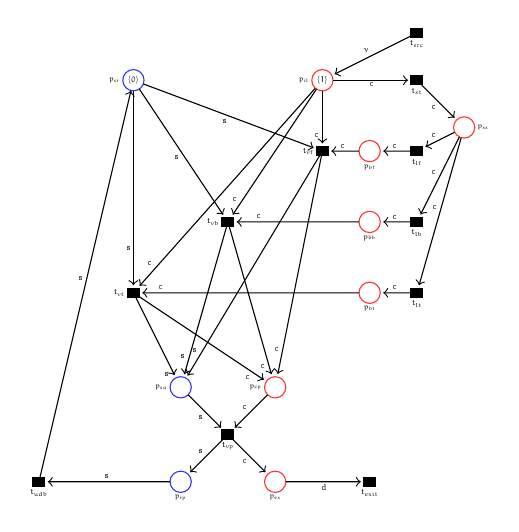
\begin{tikzpicture}[scale=0.3, transform shape]
    \centering
    \node[transition,fill=black,label=below:$t_{src}$,inner
        sep=0pt,minimum height=.40cm, minimum width=.5cm] (tsrc) at (0,1){} ;

    \node[place,draw=red!80,minimum height=.4cm,minimum width=.9cm,label=left:{\small $p_{il}$}] (pil) at (-4,-1) {$\{1\}$} edge[pre] node[auto] {$\nu$} (tsrc);

    \node[place,draw=blue!80,minimum height=.4cm,minimum width=.9cm,label=left:{\small $p_{sr}$}] (psr) at (-12,-1) {$\{0\}$};

    \node[transition,fill=black,label=below:$t_{st}$,inner
        sep=0pt,minimum height=.40cm, minimum width=.5cm] (tst) at (0,-1){} edge[pre] node[auto] {c} (pil);
    \node[place,draw=red!80,minimum height=.4cm,minimum width=.9cm,label=right:{\small $p_{ss}$}] (pss) at (2,-3) {} edge[pre] node[auto] {c} (tst);
    \node[transition,fill=black,label=below:$t_{lf}$,inner
        sep=0pt,minimum height=.40cm, minimum width=.5cm] (tlf) at (0,-4){} edge[pre] node[auto] {c} (pss);
    \node[place,draw=red!80,minimum height=.4cm,minimum width=.9cm,label=below:{\small $p_{bf}$}] (pbf) at (-2,-4) {} edge[pre] node[auto] {c} (tlf);
    \node[transition,fill=black,label=left:$t_{vf}$,inner
        sep=0pt,minimum height=.40cm, minimum width=.5cm] (tvf) at (-4,-4){} edge[pre] node[auto] {c} (pbf) edge[pre] node[auto,pos=0.2] {c} (pil) edge[pre] node[auto] {s} (psr);


    \node[transition,fill=black,label=below:$t_{lb}$,inner
        sep=0pt,minimum height=.40cm, minimum width=.5cm] (tlb) at (0,-7){} edge[pre] node[auto] {c} (pss);
    \node[place,draw=red!80,minimum height=.4cm,minimum width=.9cm,label=below:{\small $p_{bb}$}] (pbb) at (-2,-7) {} edge[pre] node[auto] {c} (tlb);
    \node[transition,fill=black,label=left:$t_{vb}$,inner
        sep=0pt,minimum height=.40cm, minimum width=.5cm] (tvb) at (-8,-7){} edge[pre] node[auto,pos=0.2] {c} (pbb) edge[pre] node[auto,pos=0.1] {c} (pil) edge[pre] node[auto] {s} (psr);


    \node[transition,fill=black,label=below:$t_{lt}$,inner
        sep=0pt,minimum height=.40cm, minimum width=.5cm] (tlt) at (0,-10){} edge[pre] node[auto] {c} (pss);
    \node[place,draw=red!80,minimum height=.4cm,minimum width=.9cm,label=below:{\small $p_{bt}$}] (pbt) at (-2,-10) {} edge[pre] node[auto] {c} (tlt);
    \node[transition,fill=black,label=left:$t_{vt}$,inner
        sep=0pt,minimum height=.40cm, minimum width=.5cm] (tvt) at (-12,-10){} edge[pre] node[auto,pos=0.1] {c} (pbt) edge[pre] node[auto,pos=0.1] {c} (pil) edge[pre] node[auto,pos=0.2] {s} (psr);

    \node[place,draw=blue!80,minimum height=.4cm,minimum width=.9cm,label=left:{\small $p_{sa}$}] (psa) at (-10,-14) {}
    edge[pre] node[auto,pos=0.1] {s} (tvf)
    edge[pre] node[auto,pos=0.1] {s} (tvb)
    edge[pre] node[auto,pos=0.1] {s} (tvt);


    \node[place,draw=red!80,minimum height=.4cm,minimum width=.9cm,label=left:{\small $p_{cp}$}] (pcp) at (-6,-14) {}
    edge[pre] node[auto,pos=0.1] {c} (tvf)
    edge[pre] node[auto,pos=0.1] {c} (tvb)
    edge[pre] node[auto,pos=0.1] {c} (tvt);

    \node[transition,fill=black,label=below:$t_{vp}$,inner
        sep=0pt,minimum height=.40cm, minimum width=.5cm] (tvp) at (-8,-16){}
    edge[pre] node[auto,pos=0.5] {s} (psa)
    edge[pre] node[auto,pos=0.5] {c} (pcp);

    \node[place,draw=blue!80,minimum height=.4cm,minimum width=.9cm,label=below:{\small $p_{rp}$}] (prp) at (-10,-18) {}
    edge[pre] node[auto,pos=0.5] {s} (tvp);


    \node[place,draw=red!80,minimum height=.4cm,minimum width=.9cm,label=below:{\small $p_{es}$}] (pes) at (-6,-18) {}
    edge[pre] node[auto,pos=0.5] {c} (tvp);


    \node[transition,fill=black,label=below:$t_{exit}$,inner
        sep=0pt,minimum height=.40cm, minimum width=.5cm] (texit) at (-2,-18){}
    edge[pre] node[auto] {d} (pes);

    \node[transition,fill=black,label=below:$t_{udb}$,inner
        sep=0pt,minimum height=.40cm, minimum width=.5cm] (tudb) at (-16,-18){}
    edge[pre] node[auto] {s} (prp)
    edge[->] node[auto] {s} (psr);

\end{tikzpicture}

}
        \scalebox{0.3}{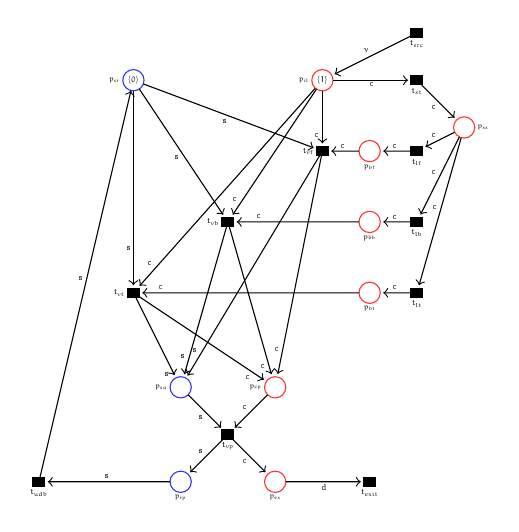
\begin{tikzpicture}[scale=0.3, transform shape]
    \centering
    \node[transition,fill=black,label=below:$t_{src}$,inner
        sep=0pt,minimum height=.40cm, minimum width=.5cm] (tsrc) at (0,1){} ;

    \node[place,draw=red!80,minimum height=.4cm,minimum width=.9cm,label=left:{\small $p_{il}$}] (pil) at (-4,-1) {$\{1\}$} edge[pre] node[auto] {$\nu$} (tsrc);

    \node[place,draw=blue!80,minimum height=.4cm,minimum width=.9cm,label=left:{\small $p_{sr}$}] (psr) at (-12,-1) {$\{0\}$};

    \node[transition,fill=black,label=below:$t_{st}$,inner
        sep=0pt,minimum height=.40cm, minimum width=.5cm] (tst) at (0,-1){} edge[pre] node[auto] {c} (pil);
    \node[place,draw=red!80,minimum height=.4cm,minimum width=.9cm,label=right:{\small $p_{ss}$}] (pss) at (2,-3) {} edge[pre] node[auto] {c} (tst);
    \node[transition,fill=black,label=below:$t_{lf}$,inner
        sep=0pt,minimum height=.40cm, minimum width=.5cm] (tlf) at (0,-4){} edge[pre] node[auto] {c} (pss);
    \node[place,draw=red!80,minimum height=.4cm,minimum width=.9cm,label=below:{\small $p_{bf}$}] (pbf) at (-2,-4) {} edge[pre] node[auto] {c} (tlf);
    \node[transition,fill=black,label=left:$t_{vf}$,inner
        sep=0pt,minimum height=.40cm, minimum width=.5cm] (tvf) at (-4,-4){} edge[pre] node[auto] {c} (pbf) edge[pre] node[auto,pos=0.2] {c} (pil) edge[pre] node[auto] {s} (psr);


    \node[transition,fill=black,label=below:$t_{lb}$,inner
        sep=0pt,minimum height=.40cm, minimum width=.5cm] (tlb) at (0,-7){} edge[pre] node[auto] {c} (pss);
    \node[place,draw=red!80,minimum height=.4cm,minimum width=.9cm,label=below:{\small $p_{bb}$}] (pbb) at (-2,-7) {} edge[pre] node[auto] {c} (tlb);
    \node[transition,fill=black,label=left:$t_{vb}$,inner
        sep=0pt,minimum height=.40cm, minimum width=.5cm] (tvb) at (-8,-7){} edge[pre] node[auto,pos=0.2] {c} (pbb) edge[pre] node[auto,pos=0.1] {c} (pil) edge[pre] node[auto] {s} (psr);


    \node[transition,fill=black,label=below:$t_{lt}$,inner
        sep=0pt,minimum height=.40cm, minimum width=.5cm] (tlt) at (0,-10){} edge[pre] node[auto] {c} (pss);
    \node[place,draw=red!80,minimum height=.4cm,minimum width=.9cm,label=below:{\small $p_{bt}$}] (pbt) at (-2,-10) {} edge[pre] node[auto] {c} (tlt);
    \node[transition,fill=black,label=left:$t_{vt}$,inner
        sep=0pt,minimum height=.40cm, minimum width=.5cm] (tvt) at (-12,-10){} edge[pre] node[auto,pos=0.1] {c} (pbt) edge[pre] node[auto,pos=0.1] {c} (pil) edge[pre] node[auto,pos=0.2] {s} (psr);

    \node[place,draw=blue!80,minimum height=.4cm,minimum width=.9cm,label=left:{\small $p_{sa}$}] (psa) at (-10,-14) {}
    edge[pre] node[auto,pos=0.1] {s} (tvf)
    edge[pre] node[auto,pos=0.1] {s} (tvb)
    edge[pre] node[auto,pos=0.1] {s} (tvt);


    \node[place,draw=red!80,minimum height=.4cm,minimum width=.9cm,label=left:{\small $p_{cp}$}] (pcp) at (-6,-14) {}
    edge[pre] node[auto,pos=0.1] {c} (tvf)
    edge[pre] node[auto,pos=0.1] {c} (tvb)
    edge[pre] node[auto,pos=0.1] {c} (tvt);

    \node[transition,fill=black,label=below:$t_{vp}$,inner
        sep=0pt,minimum height=.40cm, minimum width=.5cm] (tvp) at (-8,-16){}
    edge[pre] node[auto,pos=0.5] {s} (psa)
    edge[pre] node[auto,pos=0.5] {c} (pcp);

    \node[place,draw=blue!80,minimum height=.4cm,minimum width=.9cm,label=below:{\small $p_{rp}$}] (prp) at (-10,-18) {}
    edge[pre] node[auto,pos=0.5] {s} (tvp);


    \node[place,draw=red!80,minimum height=.4cm,minimum width=.9cm,label=below:{\small $p_{es}$}] (pes) at (-6,-18) {}
    edge[pre] node[auto,pos=0.5] {c} (tvp);


    \node[transition,fill=black,label=below:$t_{exit}$,inner
        sep=0pt,minimum height=.40cm, minimum width=.5cm] (texit) at (-2,-18){}
    edge[pre] node[auto] {d} (pes);

    \node[transition,fill=black,label=below:$t_{udb}$,inner
        sep=0pt,minimum height=.40cm, minimum width=.5cm] (tudb) at (-16,-18){}
    edge[pre] node[auto] {s} (prp)
    edge[->] node[auto] {s} (psr);

\end{tikzpicture}

}
        % \caption{Travel Agency Case Study}
        % \label{fig:travelnunet}
    \end{figure}
\end{frame}

\begin{frame}{Bounded Semantics}
    $M,[x\mapsto a],i\models^{k}_x \mathbf{F}_c\alpha$ iff\\
    $\exists j: i \le j \le k$, $a\in V_j$ and $M,[x\mapsto a],j\models^{k}_x \alpha$.


    \begin{columns}[T]
        \begin{column}{.5\textwidth}
            \begin{figure}
                \begin{center}
                    \scalebox{0.8}{\input{figures/live_windows_overlap_line_3}}
                \end{center}
                \caption{Snapshot with 4 clients}
                \label{fig:4clients}
            \end{figure}
        \end{column}
        \hfill
        \begin{column}{.5\textwidth}
            \begin{figure}
                \begin{center}
                    \scalebox{0.8}{\input{figures/live_windows_overlap_line}}
                \end{center}
                \caption{Snapshot with 2 clients}
                \label{fig:2clients}
            \end{figure}
        \end{column}
    \end{columns}
    Given $\alpha=PR(x)$. The above formula is satisfiable for all clients in both figures.
\end{frame}
\end{document}
% \endinput